% document formatting
\documentclass[10pt]{article}
\usepackage[utf8]{inputenc}
\usepackage[left=1in,right=1in,top=1in,bottom=1in]{geometry}
\usepackage[T1]{fontenc}
\usepackage{xcolor}

% math symbols, etc.
\usepackage{amsmath, amsfonts, amssymb, amsthm}
\usepackage{dsfont}

% lists
\usepackage{enumerate}

% images
\usepackage{graphicx} % for images
\usepackage{tikz}
\usetikzlibrary{fit}

% code blocks
\usepackage{minted, listings} 

% verbatim greek
\usepackage{alphabeta}
\DeclareMathOperator*{\argmin}{arg\,min}
\DeclareMathOperator*{\argmax}{arg\,max}

\graphicspath{{./assets/images/}}

\title{02-750 Week 3 \\ \large{Automation of Scientific Research}}
 
\author{Aidan Jan}

\date{\today}

\begin{document}
\maketitle

\section*{Artificial Intelligence}
Note that machine learning is a subset of artificial intelligence.  Deep learning is a subset of machine learning.

\subsection*{What is Artificial Intelligence (AI)?}
``Any task performed by a machine that would have previously been considered to require human intelligence.'' - Professors Mavin Minsky and John McCarthy (1956)
\begin{itemize}
	\item ``It is the science and engineering of making intelligent machines, especially intelligent computer programs.  It is related to the similar task of using computers to understand human intelligence, but AI does not have to confine itself to methods that are biologically observable.'' - Professor John McCarthy (2004)
	\item ``A system's ability to adapt and improvise in a new environment, to generalize its knowledge and apply it to unfamiliar scenarios.'' - AI researcher Fran\c{c}ais (2020)
\end{itemize}

\subsection*{What is Machine Learning (ML)?}
\begin{itemize}
	\item A branch of AI
	\item ``Study of computer \textbf{algorithms} that allow computer programs to automatically \textbf{improve} through \textbf{experience}.'' - Prof. Tom Mitchell (1997)
\end{itemize}
\begin{center} 
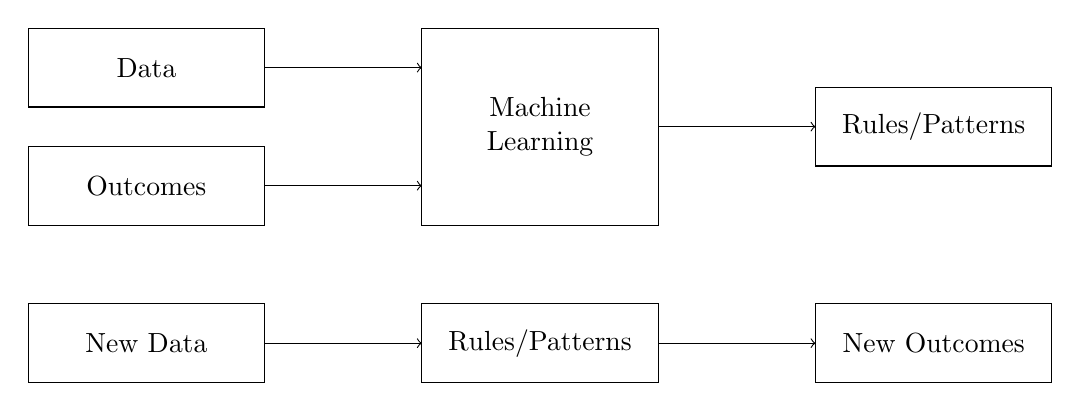
\begin{tikzpicture}
    \draw (0, 4) rectangle (3, 3) node[midway] {Data};
    \draw (0, 2.5) rectangle (3, 1.5) node[midway] {Outcomes};
    \draw (5, 4) rectangle (8, 1.5) node[midway, align=center] {Machine\\Learning};
    \draw (10, 3.25) rectangle (13, 2.25) node[midway] {Rules/Patterns};

    \draw (0, 0.5) rectangle (3, -0.5) node[midway] {New Data};
    \draw (5, 0.5) rectangle (8, -0.5) node[midway] {Rules/Patterns};
    \draw (10, 0.5) rectangle (13, -0.5) node[midway] {New Outcomes};
    
    \draw[->] (3, 3.5) -- (5, 3.5);
    \draw[->] (3, 2) -- (5, 2);
    \draw[->] (8, 2.75) -- (10, 2.75);
    \draw[->] (3, 0) -- (5, 0);
    \draw[->] (8, 0) -- (10, 0);
\end{tikzpicture}
\end{center}

\subsection*{Types of Machine Learning}
\begin{itemize}
	\item Supervised Learning
	\begin{itemize}
	    \item Input: Training data and labels.
	    \item Goal: Learn function to map new unlabelled data to labels.
	    \item For example, classification and regression.
    \end{itemize}
	\item Semi-Supervised Learning
	\begin{itemize}
	    \item Input: Training data, some of which is labelled.
	    \item Goal: Learn function to map new unlabelled data to labels and/or learn structure in the data.
    \end{itemize}
	\item Reinforcement Learning
	\begin{itemize}
	    \item Given a sequence of states and actions with (delayed) rewards, output a policy
	    \item Policy is a mapping from states to actions that tells you what to do in a given state.
	    \item Agent and environment interact at discrete time steps.  Agent commits ana action on the environment, which changes its state and rewards (either positively or negatively) the agent.
	    \item For example, training a self-driving car.
    \end{itemize}
	\item Unsupervised Learning
	\begin{itemize}
	    \item Input: Training data without labels.
	    \item Goal: Learn structure in the data.
	    \item For example, K-means Clustering
    \end{itemize}
\end{itemize}

\subsection*{When to Use Machine Learning}
Machine Learning is used when:
\begin{itemize}
	\item human expertise does not exist (e.g., navigating on Mars)
	\item humans can't explain their expertise (e.g., speech recognition)
	\item models must be customized (e.g., personalized medicine)
	\item models are based on huge amounts of data (e.g., genomics)
\end{itemize}
Learning isn't always useful:
\begin{itemize}
	\item There is no need to "learn" to calculate payroll
\end{itemize}

\subsection*{Designing a Learning System}
\begin{itemize}
	\item Choose the training experience
	\item Choose exactly what is to be learned (i.e., the \textit{target function})
	\item Choose how to represent the target function
	\item Choose a learning algorithm to infer the target function from the experience
\end{itemize}

\subsection*{Training vs. Test Distribution}
\begin{itemize}
	\item We generally assume that the training and test examples are independently drawn from the same overall distribution of data
	\begin{itemize}
	    \item We call this ``i.i.d'' which stands for ``independent and identically distributed''
    \end{itemize}
    \item If examples are not independent, it requires \textit{collective classification}.
    \item If the test distribution is different, it requires \textit{transfer learning}.
\end{itemize}

\subsection*{ML in a Nutshell}
\begin{itemize}
	\item Tens of thousands of machine learning algorithms.  (Hundreds of new ones every year)
	\item Every ML algorithm has three components:
	\begin{itemize}
	    \item Representation
	    \item Optimization
	    \item Evaluation
    \end{itemize}
    \item Deep Learning tends to do better than most machine learning algorithms when the amount of data grows large.
\end{itemize}

\subsection*{Various Function Representations}
\begin{itemize}
	\item Numerical functions
	\begin{itemize}
	    \item Linear Regression
	    \item Neural Networks
	    \item Support Vector Machines
    \end{itemize}
    \item Symbolic functions
    \begin{itemize}
	    \item Decision trees
	    \item Rules in propositional logic
	    \item Rules in first-order predicate logic
    \end{itemize}
    \item Instance-based functions
    \begin{itemize}
	    \item Nearest-neighbor
	    \item Case-based
    \end{itemize}
    \item Probabilistic Graphical Models
    \begin{itemize}
	    \item Na\text{\"i}ve Bayes
	    \item Bayesian networks
	    \item Hidden-Markov Models (HMMs)
	    \item Probabilistic Context Free Grammars (PCFGs)
	    \item Markov networks
    \end{itemize}
\end{itemize}

\subsection*{Various Search / Optimization Algorithms}
\begin{itemize}
	\item Gradient Descent
	\begin{itemize}
	    \item Perceptrons
	    \item Backpropagation
    \end{itemize}
	\item Dynamic Programming
	\begin{itemize}
	    \item HMM Learning
	    \item PCFG Learning
    \end{itemize}
	\item Divide and Conquer
	\begin{itemize}
	    \item Decision tree induction
	    \item Rule learning
    \end{itemize}
	\item Evolutionary Computation
	\begin{itemize}
	    \item Genetic Algorithms (GAs)
	    \item Genetic Programming (GP)
	    \item Neuro-evolution
    \end{itemize}
\end{itemize}

\subsection*{Evaluating ML Models}
\begin{itemize}
	\item Accuracy
	\item Precision and Recall
	\item Squared Error
	\item Likelihood
	\item Posterior Probability
	\item Cost / Utility
	\item Margin
	\item Entropy
	\item K-L Divergence
	\item etc.
\end{itemize}





\end{document}